
\chapter{Background and Related Works}

\section{Background overview}

The task of determining the position of an object in space is not new. Over the past 20 years, a large number of works have been aimed at solving this problem \cite{6, 7}. A lot has changed with the advent of depth sensors and neural networks. These technologies introduce new approaches to comprehensive scene analysis. Depth cameras produce information about the distance to an object, which allows reconstructions of more accurate 3D models, and neural networks calculate complex correlations in image patterns. Since 2012, neural networks started to overperform most of the classical methods in segmentation and classification problems. A large number of methods use a combination of depth-camera output and neural network for 3D reconstruction of the body position \cite{8, 9}. The above technologies also apply widely to the hands. Often, researchers use a combination of depth sensors and gloves, which record the 3D position of the hand. Several sensors are used for the collection of fully labeled training samples for 3D reconstruction, which may include depth map, joint angles, and 3D positions \cite{1,2,3}.  

Because we are solving the problem without the usage of depth sensors, from two stated technologies, we will provide only neural networks review.

\subsection{An artificial neural networks} 

An artificial neural network is a mathematical model well suited for the approximation of highly nonlinear functions. The main component of a neural network is a neuron, which usually consists of a linear regression followed by the activation function. Activation functions are responsible for the addition of nonlinear transformations. Neurons can be combined into various layers, for example, fully connected layers or convolutional layers. 

Neurons in a fully connected layer extend the idea of a linear model, where output is a linear combination of fixed nonlinear basis functions \(\phi(.)\), passed to the nonlinear activation \(f(.)\) \cite{BISHOP}:
\begin{equation}
y(x,w) = f(\sum_{j=1}^{M}w_{j}\phi_{j}(x))
\end{equation}
The extension of the idea consists of two facts. First is that nonlinear basis function is parametrized too and optimized alongside parameters {w}. Second is that basis function has the same form as 5.1.\cite{BISHOP}

The basic neural network model can be described as a series of functional transformations. First, we construct M linear combinations of the input variables $x_1, …, x_D$ in the following form:
\begin{equation}
a_j = \sum_{i=1}^{D}w_{ji}^{(1)}x_i+2_{j0}^{(1)}
\end{equation}
where j = 1, …, M, and the superscript (1) indicates that the corresponding parameters are in the first ‘layer’ of the network.
The output of 2.2 called activation and transformed using a differentiable, nonlinear activation function h(.):
\begin{equation}
z_j = h(a_j)
\end{equation}
where $z_j$ is called hidden unit.

A popular choice of an activation function for multiple binary classification problems is a sigmoidal activation. It is a convenient activation function for computer vision tasks such as image segmentation or key-points detection:
\begin{equation}
\sigma(a) = \frac{1}{1 + exp(-a)}
\end{equation}
So then, a multilayer neural network with sigmoidal activation function can be represented by the equation 2.5:
\begin{equation}
y_k(x,w) = \sigma\left(\sum_{j=1}^{M}w_{kj}^{(2)}h\left(\sum_{i=1}^{D}w_{ji}^{(1)}x_i + w_{k0}^{(1)}\right)+w_{k0}^{(2)}\right)
\end{equation}
where w is a matrix of all trainable parameters \cite{BISHOP}. 

Convolutional layers are a fundamental part of most networks described in this thesis. The core component of a layer is the sliding kernel matrix (filter) with trainable parameters. Elements of the kernel matrix multiplied element-wise with a region of the input matrix. The following equation describes the process:
\begin{equation}
G[m,n] = (f*h)[m,n] = \sum_{j}\sum_{k}h[j,k]f[m-j,n-k]
\end{equation}
where f - is an input matrix, h kernel, m - rows, n - columns 

Multiplication results are summated with bias, and output is represented as an element of the feature map matrix. Feature map usually transformed with some activation function. Because for one feature map exist only one kernel matrix with trainable parameters, a number of weights are significantly smaller than in a fully connected layer. The trainable convolution can be described as linear regression trained on segments of the input data, not all data at once. By changing the dimension of the kernel or sparseness of the input region, we can determine the logic of pattern recognition performed by the layer.

\begin{figure}
\caption{Conv}
\centering
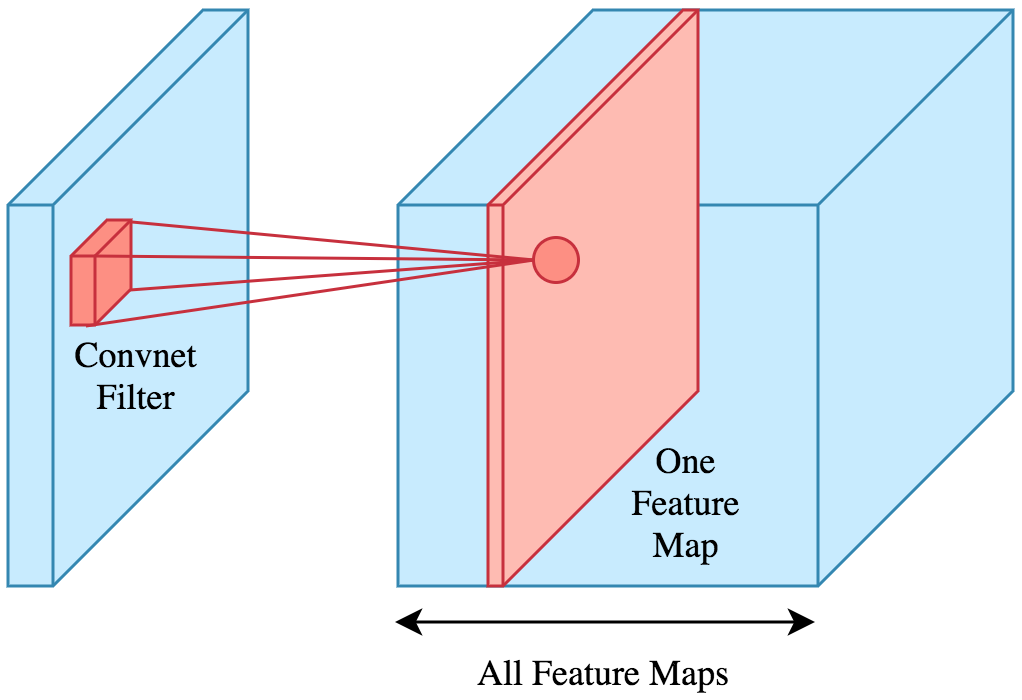
\includegraphics[width=0.5\textwidth]{pic_conv}
\end{figure}

In the simplest case, the trainable parameters of the network are only weights of a linear regression that optimized using gradient descent. Various techniques, such as batch normalization, dropout, or skip connections, are used to prevent overfitting or speed up the optimization of parameters.

In all the reviewed and proposed methods for 3D hand modeling, convolutional neural networks (CNNs) play an essential role.

\subsection{Blocks and cells}

In this section, we review two structures built from layers. Both of them mainly solve the problem of vanishing gradient. The first one is called residual block and was introduced as a solution for efficient training of deep networks with depth in hundreds of layers \cite{24} . Residual block returns not the output of the single final layer but the sum of multiple outputs. This design allows the optimizer to update weight at the beginning of the network more efficiently.

\begin{figure}
\caption{Residual learning: a building block \cite{24}.}
\centering
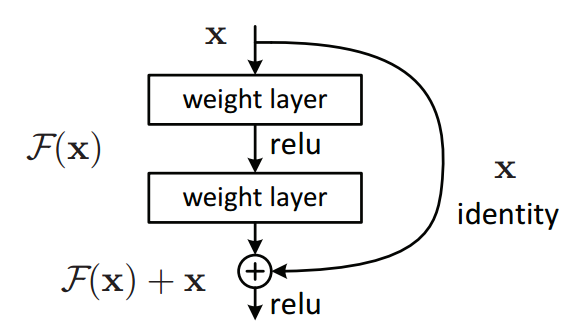
\includegraphics[width=0.5\textwidth]{res_block}
\end{figure}


The second structure is called LSTM cell and related to Recurrent Neural Networks that weren’t touched before in a thesis. RNNs are used for sequence modeling where there is a task of mapping one sequence to another. Each element of a sequence is fed to network cell, which extracts patterns of elements. The problem, in this case, again vanishing gradient for the case of long sequences and can be solved by LSTM cell. The sequence of computational operations is listed on equations 2.7-2.12 and illustrated on Fig 2.3.

\begin{figure}[h]
\caption{LSTM cell}
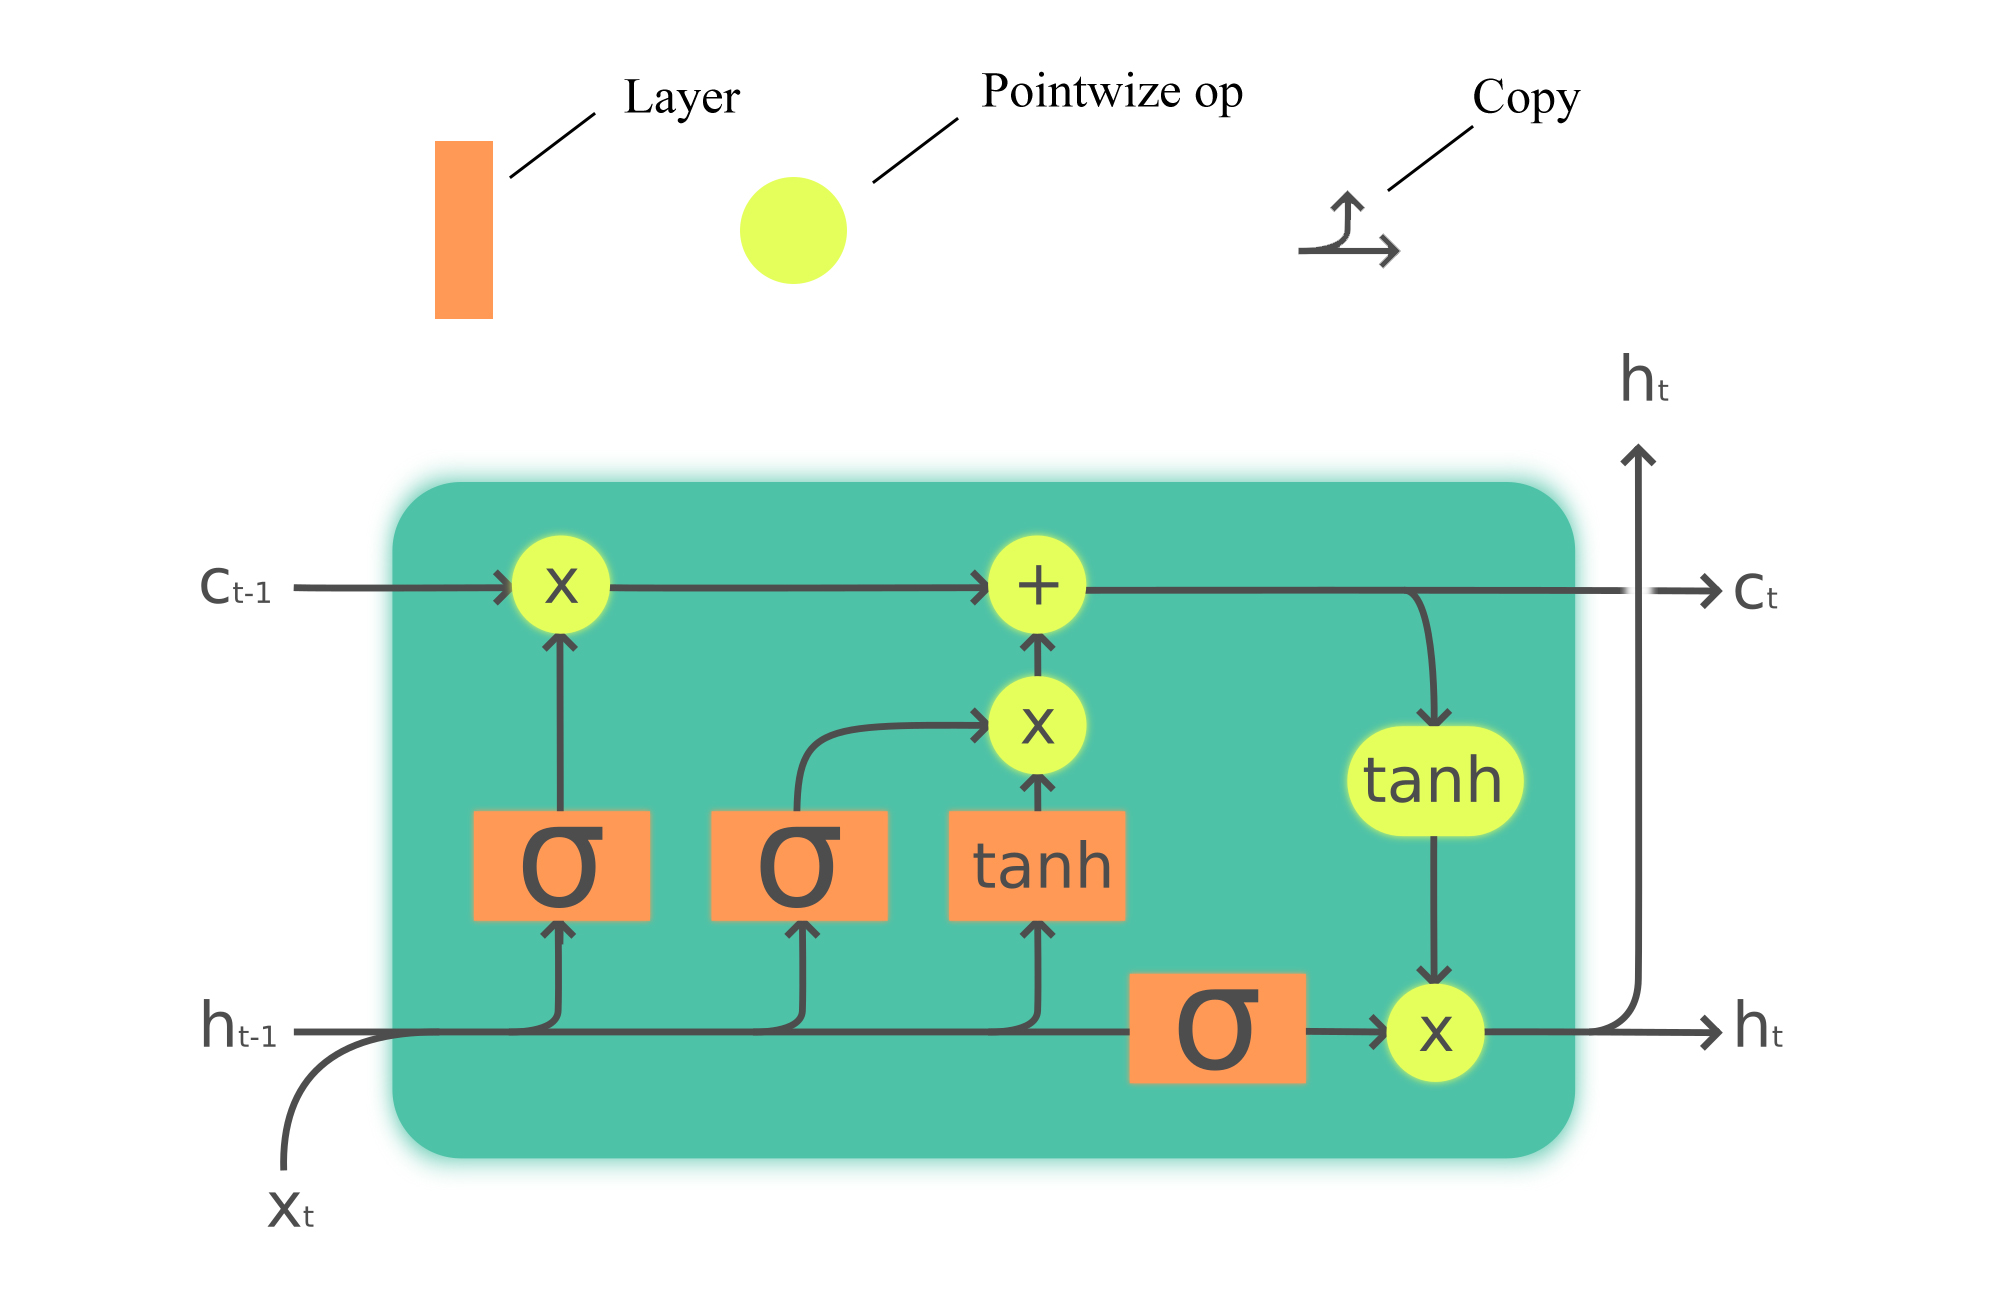
\includegraphics[width=1\textwidth]{lstm}
\end{figure}


\begin{equation}
f_t = \sigma_g(W_fx_t + U_fh_{t-1} + b_f)
\end{equation}


\begin{equation}
i_t = \sigma_g(W_ix_t + U_ih_{t-1} + b_i)
\end{equation}

\begin{equation}
o_t = \sigma_g(W_ox_t + U_oh_{t-1} + b_o)
\end{equation}

\begin{equation}
o_t = \sigma_g(W_ox_t + U_oh_{t-1} + b_o)
\end{equation}

\begin{equation}
c_t = f_t\circ c_{t-1} + i_t \circ \sigma_c(W_cx_t + U_ch_{t-1} + b_c)
\end{equation}

\begin{equation}
h_t = o_t\circ \sigma_h(c_t)
\end{equation}

\section{Methods for 3D shape estimation}

Most methods for 3D hand pose generation from a single RGB image can be generalized into four stages. The first stage is the detection of hands in the input image and cropping localized area; the second is the detection of hand key-points in 2D; the third is a mapping of 2D locations into 3D, and the fourth is a generation of the 3D hand model.


\begin{figure}[h]
\caption{Generalized schema of 3D hand pose estimation}
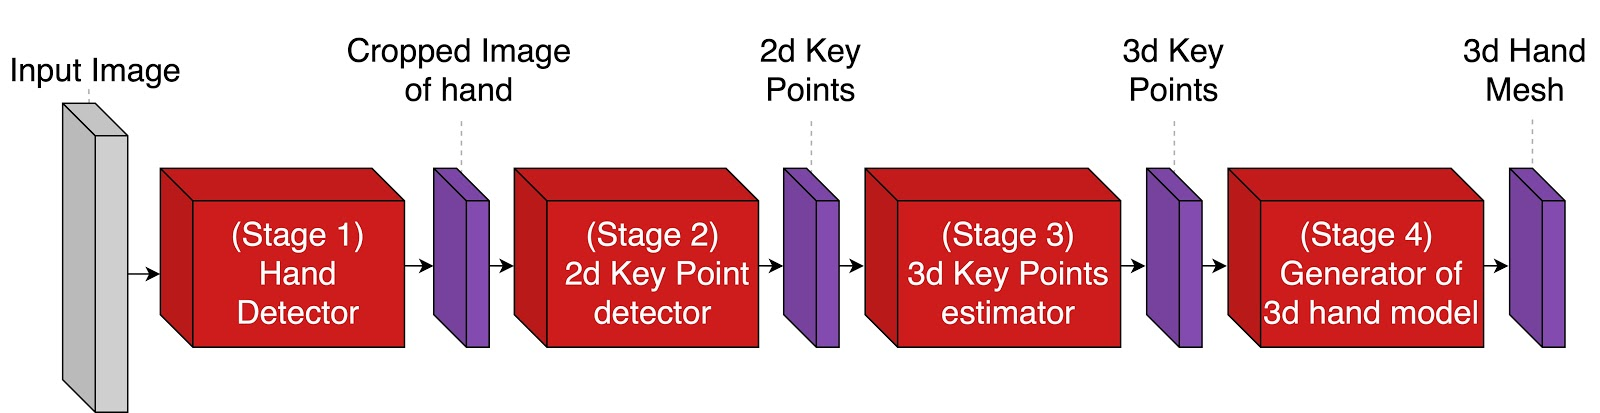
\includegraphics[width=1\textwidth]{schema3dr}
\end{figure}

\subsection{Networks for 2D key-point detection}
Estimation of 3D structures such as 3D key-points or 3D hand model is the hardest to train part of the pipeline. For higher accuracy of those stages, it is essential to accurately estimate 2D key-points of the hand, because this data contains two-thirds of the 3D locations. We will review a few models suitable to address tasks of 2D key-points estimation. We will discuss three CNNs, namely U-Net, Stacked Hourglass Network, and Open Pose. 

\begin{figure}
\caption{a) U\-Net architecture \cite{25} , b) Stacked Hourglass Network \cite{27}}
\centering
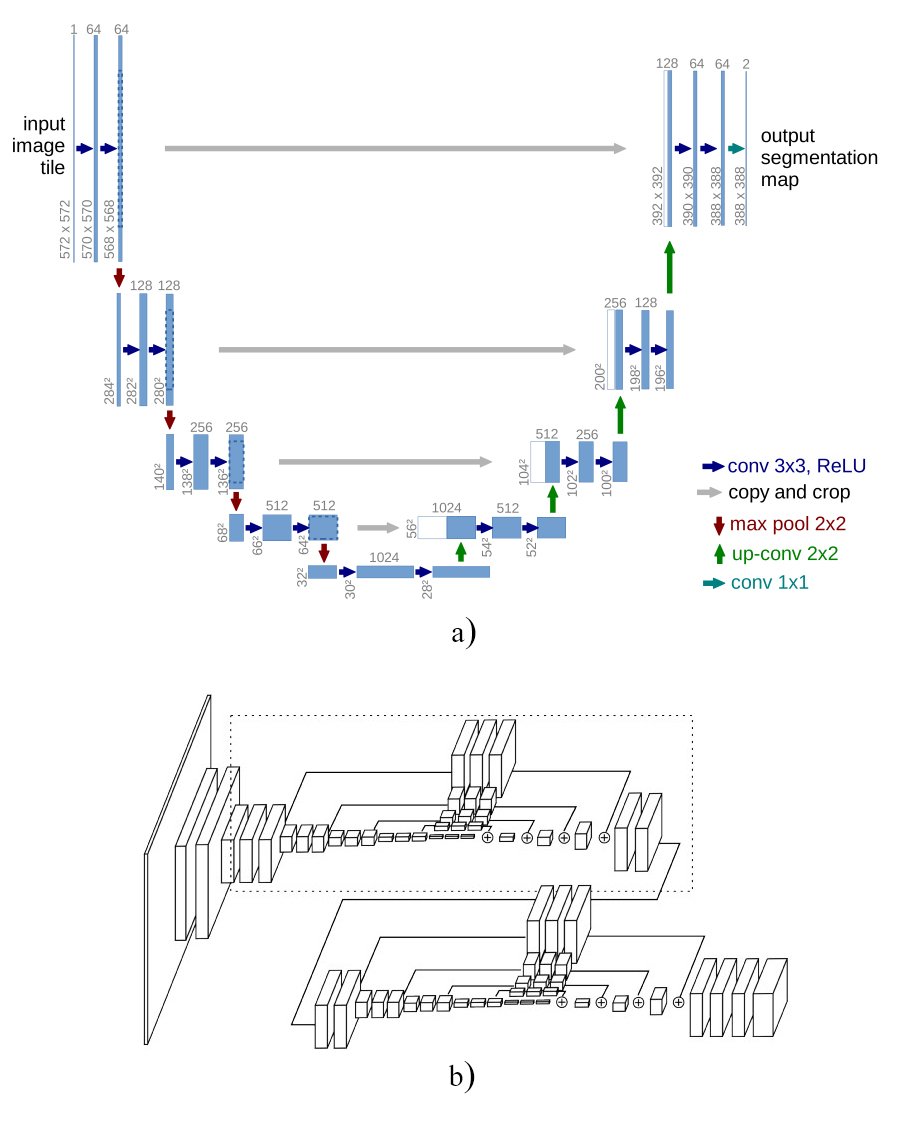
\includegraphics[width=0.7\textwidth]{nuets}
\end{figure}

The U\-Net is an architecture which first extracts image features by downsampling layers and then upsamples them alongside sequential concatenation of outputs from previous layers \cite{25}. U-Net like architectures have proven to work with the task of 2D key-points detection \cite{26}.

Stacked Hourglass Network extends the idea of U-Net and stacks several architectures of a similar type into one pipeline with supervision after each step \cite{27}. Building blocks are residual and skip connections are implemented by the addition of feature maps rather than concatenation.

Open pose detector is a CNN that consists of multiple computational stages and two parallel computational pipelines. Each stage is estimating both locations of 2D key-points and connections between them. All stages except the first one are estimating information about joints based on previous results. In such a way, the detector is reffing computational results with each iteration.

\subsection{Systems for 3D reconstruction}

The paper \cite{10} introduces a three-stage algorithm that localizes the hands and determines the key-points in 2D at the first two stages and calculates 3D reconstruction at the third is studied in the paper. 

\begin{figure}
\caption{Illustration of parallel computational pipelines used in Open Pose \cite{PCP}}
\centering
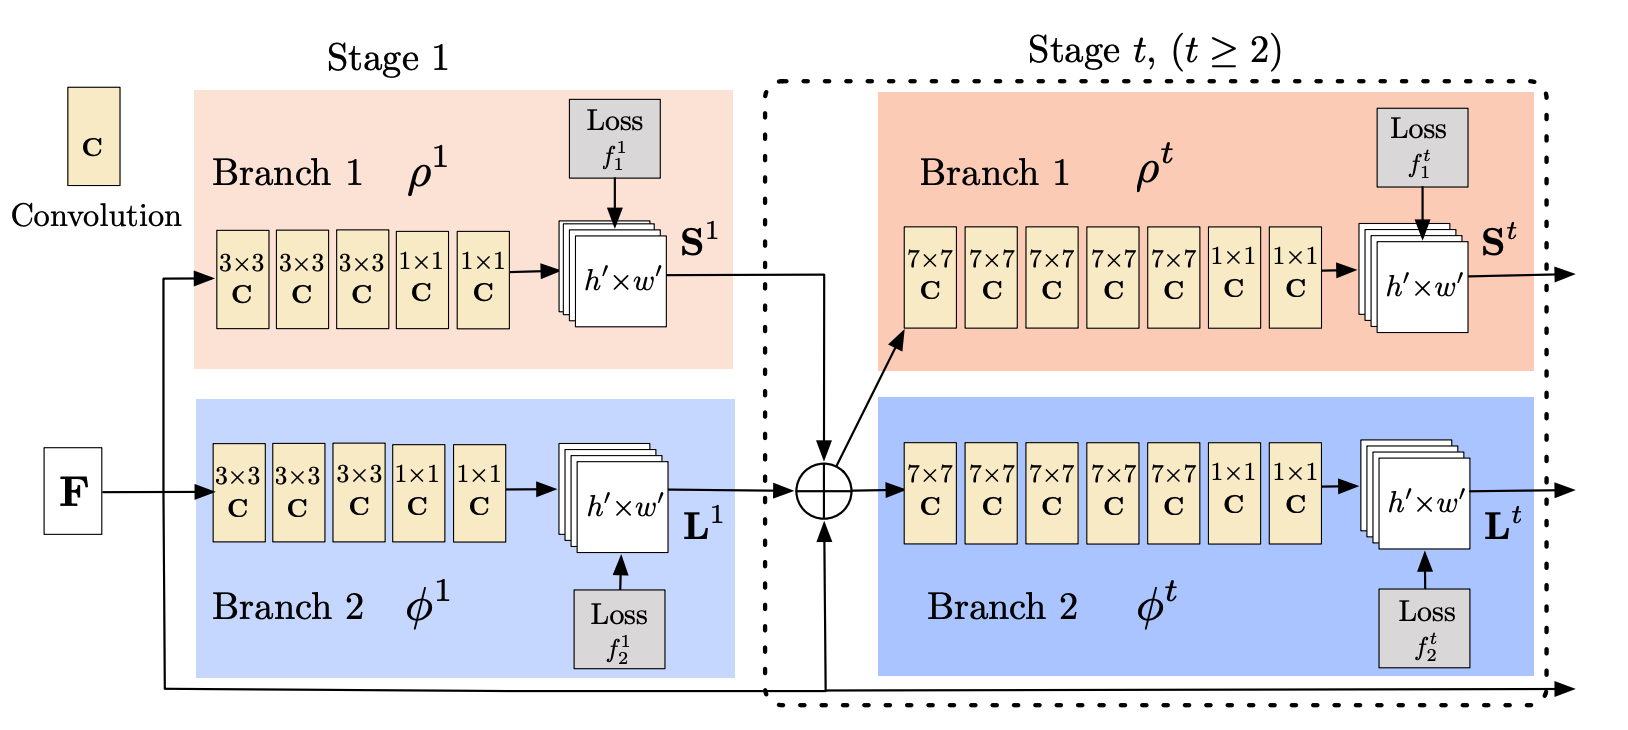
\includegraphics[width=1\textwidth]{methodPCP}
\end{figure}


The first stage is the YOLOv2 neural network (‘you only look once’), which identifies the position of the hands. YOLOv2 is a CNN which used for localization and classification of multiple objects at once.

The localized hands are passed to the OpenPose detector.

These two neural networks localize 21 2D key-points on the video frames, which are then used as a target in the inverse kinematic optimization problem. A distinct drawback of this method is the limitation caused by the error of the OpenPose detector. This error causes the algorithm to optimize 3D locations using the wrong 2D key-points. Nevertheless, the addition of a hand position from a different view makes it possible to improve the optimization problem, and hence the accuracy. The runtime of the method on Nvidia GTX 1070 GPU is close to 53 ms. 

The work \cite{23} describes one of the few methods which fully reconstructs the 3D shape of the hand. It introduces a graph convolutional neural network (CNN) for generating 3D mesh. The work uses centered images of hands as input, thus hand detection was not necessary. Therefore, the first part of the approach is 2D key-point detection, which is based on Stacked Hourglass Networks. The second is the encoding of 2D features, and the third is 3D reconstruction with a graph CNN network. The network outperforms state-of-the-art methods on RHD \cite{13} and STB \cite{14} datasets. The runtime of the method on Nvidia GTX 1080 GPU is, on average, 19.9ms. The pretrained model is available, but the training dataset is not.

\begin{figure}
\caption{Scheme of the method described in paper 3D Hand Shape and Pose Estimation from a Single RGB Image. \cite{23}}
\centering
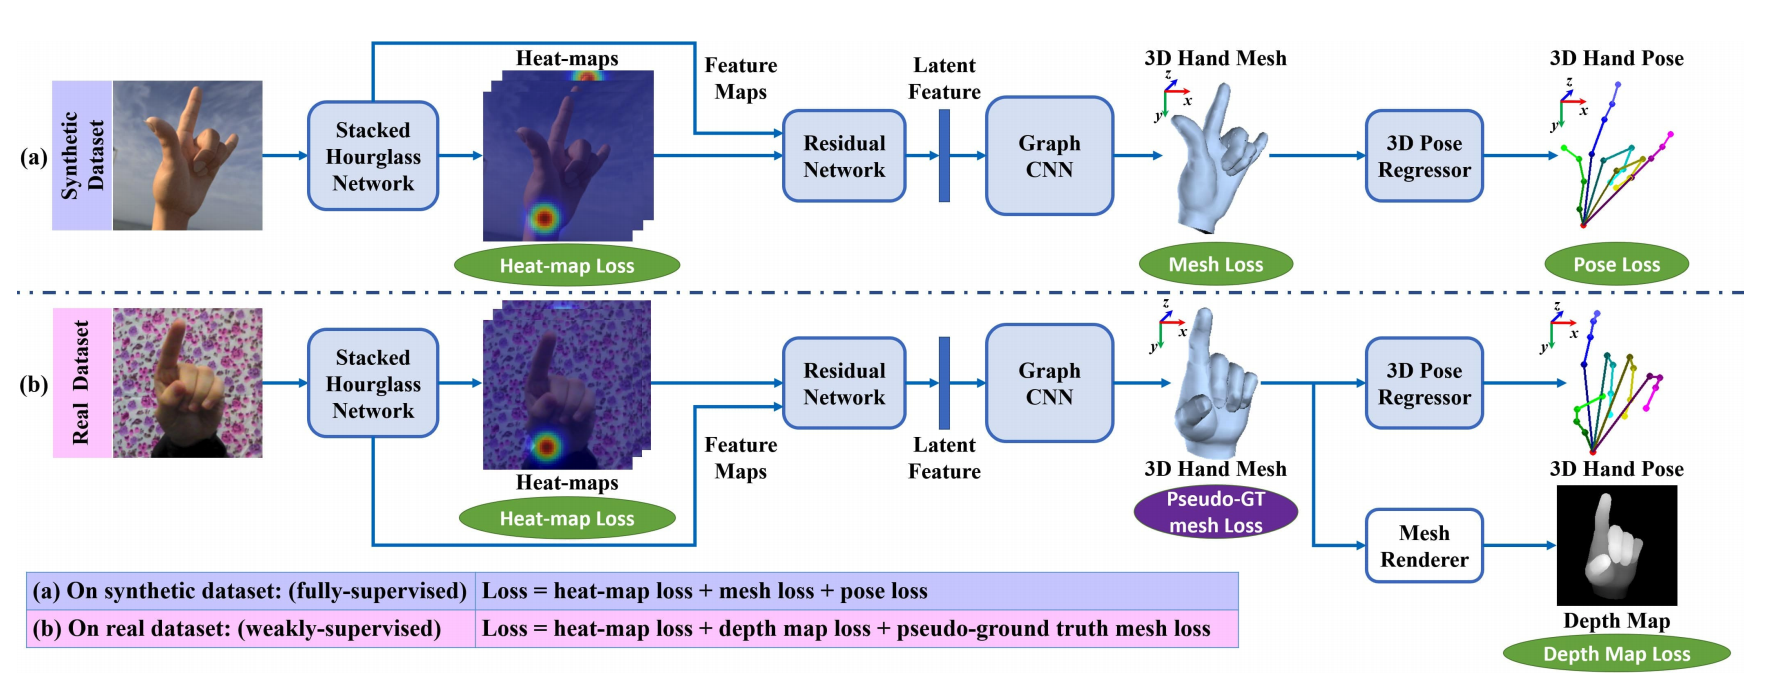
\includegraphics[width=1\textwidth]{method2}
\end{figure}

\subsection{MANO model}

MANO is a differentiable parametric model of the hand, which can be integrated into computational pipelines. MANO learned from around 1000 3D scans of hands in various poses. The model takes as input parameters of pose and shape, which then mapped to the cloud of points, which represent the hand surface \cite{MANO:SIGGRAPHASIA:2017}.